% Figure 3: Sakoe-Chiba Constrained DTW Warping Path
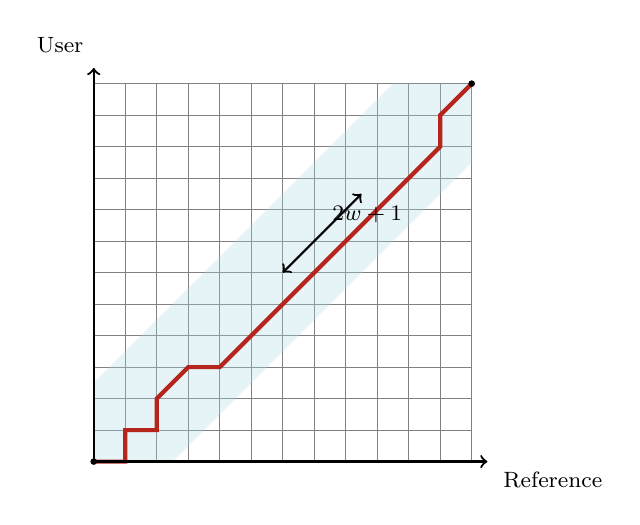
\begin{tikzpicture}[scale=0.4]

% Grid parameters
\def\N{12}
\def\M{12}
\def\w{2.5}

% Draw grid
\draw[step=1, gray, very thin] (0,0) grid (\N,\M);

% Draw Sakoe-Chiba constraint band (shaded diagonal corridor)
\fill[LightBlue, opacity=0.3]
    (0,0) -- (\w,0) -- (\N,\M-\w) -- (\N,\M) -- (\N-\w,\M) -- (0,\w) -- cycle;

% Draw optimal warping path (red line with steps)
\draw[BrickRed, line width=1.5pt]
    (0,0) -- (1,0) -- (1,1) -- (2,1) -- (2,2) -- (3,3) -- (4,3) --
    (5,4) -- (6,5) -- (7,6) -- (8,7) -- (9,8) -- (10,9) -- (11,10) --
    (11,11) -- (12,12);

% Axes
\draw[->, thick] (0,0) -- (\N+0.5,0) node[below right, xshift=2pt, font=\footnotesize] {Reference};
\draw[->, thick] (0,0) -- (0,\M+0.5) node[above left, yshift=2pt, font=\footnotesize] {User};

% Constraint width annotation (two-headed arrow)
\draw[<->, thick] (6,6) -- (6+\w,6+\w) node[midway, above right, font=\footnotesize] {$2w+1$};

% Corner markers
\fill (0,0) circle (3pt);
\fill (\N,\M) circle (3pt);

\end{tikzpicture}
